\documentclass{article}
\usepackage{geometry}                		% See geometry.pdf to learn the layout options. There are lots.
\geometry{letterpaper}                   		% ... or a4paper or a5paper or ... 
%\usepackage[parfill]{parskip}    		% Activate to begin paragraphs with an empty line rather than an indent
\usepackage{graphicx}				% Use pdf, png, jpg, or eps§ with pdflatex; use eps in DVI mode
								% TeX will automatically convert eps --> pdf in pdflatex		
\usepackage{amsmath}
%\graphicspath{{/Users/lukebury/Documents/School/CU/ORCCA/}}
\usepackage{color}
\graphicspath{{../figures/}}

\newcommand{\paragraphtitle}[1]{\paragraph{#1}\mbox{}\\}

\title{Outline - APPM 5460 Proposal Outline}
\author{Luke Bury \& Don Kuettel}


\begin{document}
\maketitle


%=======================================================================================================
\subsection{needs}
\begin{itemize}
  \item 2-4 pages
  \item Lit review
  \item dynamical system modeled by ordinary differential equations
  \item material from class\\\\\\
\end{itemize}

\subsection{outline}
\begin{itemize}
	\item Intro (don)
	  \begin{itemize}
	  	\item In this proposal, we will be investigating homoclinic orbits in the Circular Restricted Three-Body Problem
	  	\item (tie to competition history)
	  	\item Homoclinic orbits are ... 
	  	\item They are important because ...
	  \end{itemize}
	\item History w/ Lit Review (luke)
	  \begin{itemize}
	  	\item Competition basics ... 4 problems
	  	\item 1st problem was n-body problem
	  	\item Poincare went for 3-body since it was the first unsolved... settled for CR3BP 
	  	\item (description of CR3BP) (Figure \ref{fig:CR3BP_EarthMoon})
			\begin{figure}
			\centering
			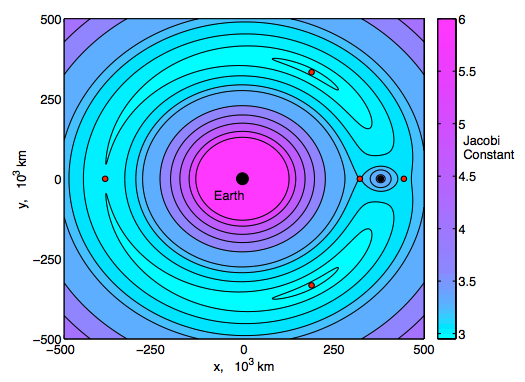
\includegraphics[scale=0.7]{CR3BP_EarthMoon.png}
			\caption{CR3BP (from CU CR3BP handout)}
			\label{fig:CR3BP_EarthMoon}
			\end{figure}
		\item
	  	\item $\ddot{x} =  2\dot{y} + x - (1-\mu)\left(\dfrac{x+\mu}{R_1^3}\right) - \mu\left(\dfrac{x-1+\mu}{R_2^3}\right)\\
		\ddot{y} = - 2\dot{x} + y\left(-\dfrac{1-\mu}{R_1^3} - \dfrac{\mu}{R_2^3} + 1\right) \\
		\ddot{z} = z\left(-\dfrac{1 - \mu}{R_1^3} - \dfrac{\mu}{R_2^3}\right)$
	  	\item (a bit on the error ... discuss the math)
	  	\item as a result, found homoclinic points/orbits

	  \end{itemize}
	\item Application w/ Lit Review
	  \begin{itemize}
	  	\item \color{red}Much research has been conducted in this field since (references, references, references)\color{black}
	  	\item (pg 72+ of book)
	  	\item we will look at / recreate Poincare's work
	  	\item we will create homoclinic orbits in the CR3BP using intersections of stable and unstable orbits in Poincare plots
	  \end{itemize}
\end{itemize}

\cite{KoonLoMarsdenRoss2011}
\bibliographystyle{plain}
\bibliography{../bibliography/appm5460.bib}

\end{document}  